\documentclass[a4paper,12pt]{scrartcl}

\usepackage[ngerman]{babel}
\usepackage[utf8]{inputenc}

%\renewcommand{\familydefault}{\sfdefault}


\usepackage[babel]{csquotes}

\newcommand{\textsub}[1]{%
	$_\text{#1}$}

\usepackage{lmodern}

\usepackage{amsmath}
\usepackage{hyperref}
\def\ra{$\rightarrow$}
\def\Ra{$\Rightarrow$}

\usepackage{siunitx}
\sisetup{tophrase={\,--\,}}
\def\idr{i.\,d.\,R.}

\usepackage{todonotes}

\usepackage{graphicx}

%\usepackage{amssymb}
%\usepackage{mathtools}
%%\usepackage{gensymb}
%\usepackage{float}

%\usepackage[a4paper, left=1cm, right=1cm, top=2cm, bottom=3cm]{geometry}

%\DeclarePairedDelimiter\abs{\lvert}{\rvert}%
%\DeclarePairedDelimiter\norm{\lVert}{\rVert}%
%\DeclarePairedDelimiter\inner{\langle}{\rangle}%
%\newcommand{\ffrac}[2]{\ensuremath{\frac{\displaystyle #1}{\displaystyle #2}}}
\usepackage{stmaryrd} % für \lightning

\begin{document}

\pagenumbering{gobble}
\title{Rechnerarchitektur Zusammenfassung}
\author{Magnus Berendes/\href{mailto:magnus.berendes@fau.de}{magnus.berendes@fau.de}}
\date{\today}
\maketitle

\newpage

\pagenumbering{Roman}

\tableofcontents
\listoftodos


\newpage
\pagenumbering{arabic}



\section{Organisation moderner RISC- und CISC-Prozessoren}

\subsection{Kurze Widerholung RISC und CISC Prinzipien}
\subsubsection{Mikroprogrammierung in CISC-Architekturen}
\begin{itemize}
	\item
		Makrobefehl bildet einstieg in Mikroprogramm

		\begin{figure}[hpbt]
			\centering
			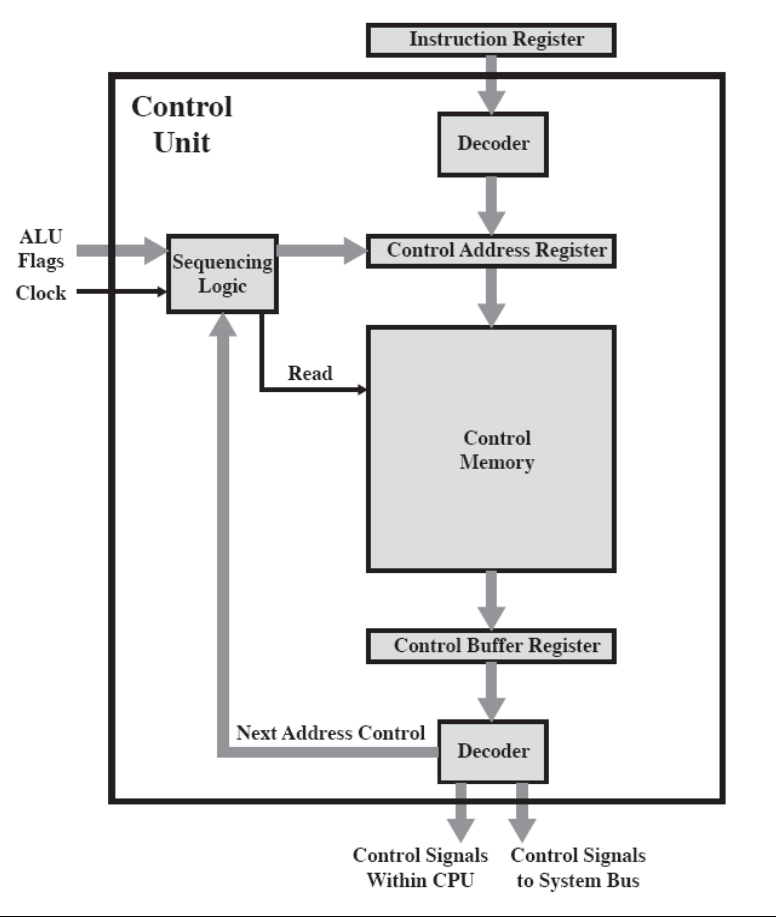
\includegraphics[width=0.5\textwidth]{img/leitwerk_mikro.png}
			\caption{Darstellung der Funktion eines mikroprogrammierten Leitwerks}
			\label{fig:mikroprog}
		\end{figure}
		\item
			Erklärung zu \autoref{fig:mikroprog}:
			\begin{itemize}
				\item
					CAR -- Control Address Register: enthält Adresse der nächsten Instruktion (1. Mikrobefehl des auszuführenden Mikroprogramms)
				\item
					CBR -- Control Buffer Register: nimmt Eintrag aus Mikroprogrammspeicher (CM) auf
				\item
					Sequencing Logic: entscheidet welche Adresse aus CM als nächstes ausgelesen wird:
					\begin{itemize}
						\item
							ALU flags (bedingter Sprung)
						\item
							Nächste Adresse: aus Adressteil des im CBR stehenden Mikrobefehls oder Inhalt CAR oder sequenzielles Fortschalten der letzten Adresse

					\end{itemize}
			\end{itemize}
		\item
			Control Memory besteht aus Sammlung von Mikroprogrammen (für fetch, für indirekte Adressierung, für Interrupts, für opcodes (AND, ADD, \dots)
		\item
			Vorteile Mikropogrammierung: 
			\begin{itemize}
				\item
					CM veränderbar $\Rightarrow$ hohe flexibilität
				\item
					Befehlskompabilität
				\item
					Andere Befehle emulieren
				\item
					Theoretisch Befehlsübersetzung mit Software $\Rightarrow$ virtuelle Maschinen
			\end{itemize}
\end{itemize}

\subsubsection{Pipelining in RISC-Architekturen}
\begin{itemize}
	\item
		Eigenschaften von RISC
		\begin{itemize}
			\item
				Prozessoren der vierten Generation
			\item
				Ziel: elementare und kleine Maschinenbefehlssätze $\Rightarrow$ Operanden und opcode holen während eines Grundtaktes ausführbar
			\item
				Addressberechnungen durch explizite Befehle, keine komplexen Adressierungsarten
			\item
				Operanden in Registern gegeben (load-store-architektur) und große universelle Registersätze
			\item
				festverdrahtete Leitwerke -- kein Mikroprogramm -- Befehl wird direkt in binäres Steuersignal dekodiert
			\item
				konsequentes Pipelining
				\begin{itemize}
					\item
						Execute aller Befehle (außer load/store) innerhalb eines Taktes ausführbar
					\item
						Wegen numerischen float Operationen nicht mehr konsequent durchzuhalten
					\item
						ab Pentium Pro wird komplexer Maschinenbefehl intern in Folge einfachere RISC Befehle zerlegt
				\end{itemize}
			\item
				Zusammenspiel von optimierenden Compiler und RISC Prozessor Arch um pipelining effizient zu nutzen

		\end{itemize}
	\item
		Durchsatz bei Pipelining im Idealfall auf $n$-fache bei $n$ Teilschritten
	\item
		Welche Leistungssteigerung möglich? 
		\begin{itemize}
			\item
				jede pipeline stufe verursacht Zusatz-Aufwand für Datenbewegung $\Rightarrow$ kritisch bei vielen Unterbrechungen im synchronen, sequentiellen Ablauf
			\item
				Mehr Steuerlogik für Register- und Speicher-Abhängigkeiten mit mehr Stufen
			\item
				Pipelinezeit durch langsamste Stufe festgesetzt
			\item
				Zykluszeit $\tau$ einer Pipeline (bestimmt Takt)
				$$
				\tau = \max_i(\tau_i) + d, \qquad d = \text{Zeitverzögerung durch Zwischenspeicherung}$$

			\item
				Erreichbarer Speed-Up $S_k$

		\end{itemize}
	\item
		Preis für Leistungssteigerung
		\begin{itemize}
			\item
				Anstieg HW-Kosten
			\item
				Anstieg Verzögerung
			\item
				Anstieg leerer Pipeline-Zyklen bei Verzweigungen
		\end{itemize}
	\item
		Heute mindestens ein Dutzen Stufen (Intel P4e: 32 Stufen)
	\item
		Weitere Entwicklung: Superskalare Recheneinheiten
		\begin{itemize}
			\item
				Erfordert mehrere Rechenwerke, heute Stand der Technik
			\item
				Gleichzeitige Anwendungen von Ops auf einzelne Komponenten eines Vektors $\Rightarrow$ superskalar
			\item
				Benötigt Befehlsgruppierer
			\item
				Umordnung sequentieller Befehle zur Laufzeit für parallel $\Rightarrow$ dynamische Parallelisierung
			\item
				Allgemeines Prinzip von superskalaren Rechnern: keine direkte Parallelität sondern Herausziehen von Parallelität aus sequentiellem Befehlsstrom
			\item
				Problem: Datenabhängigkeiten/Datenhazards

				Wenn Ergebnis von vorheriger Operation als Operand benötigt wird
			\item
				Lösung: Scoreboard und Tomasolu (siehe \ref{scoreboard} und \ref{tomasolu})
			\item
				Problem: Sprünge -- nächster Befehl in Pipeline ist gar nicht der richtige
				
		\end{itemize}

\end{itemize}

\subsection{Hazards beim Pipelining}
\begin{itemize}
	\item
		Struktur, Kontroll, Daten - Hazards
		\begin{figure}[hpbt]
			\centering
			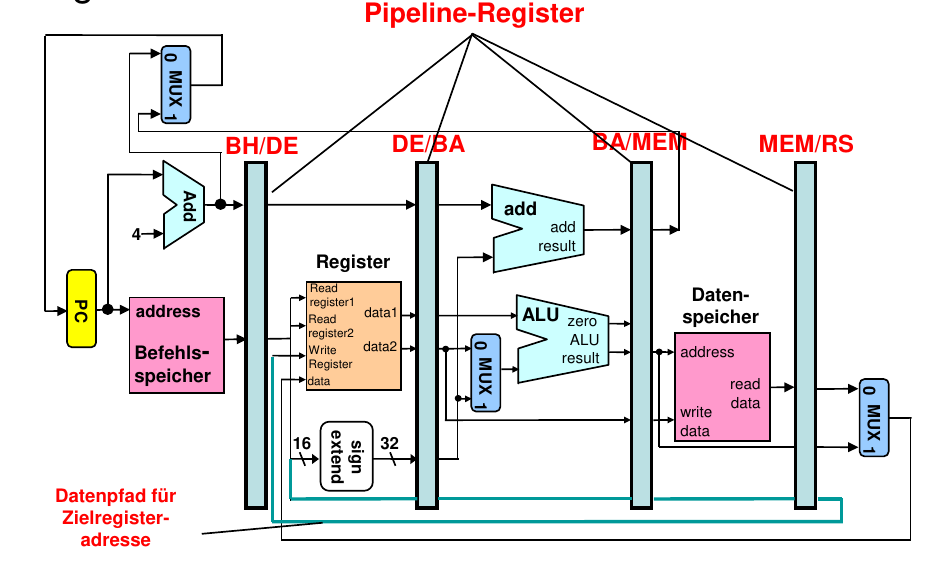
\includegraphics[width=1.1\textwidth]{img/datenpfad.png}
			\caption{Datenpfad zur Darstellung von Hazards}
			\label{fig:hazards}
		\end{figure}
	\item
		5 Phasen: Befehl Holen (BH), Befehl Dekodieren (DE),  Befehl ausführen (BA), Speicherzugriff (MEM), zurückschreiben (RS)
\end{itemize}


\subsubsection{Struktur Hazards}
\begin{itemize}
	\item
		Beispiel für strukturhazard: nur ein Speicherport, Befehl 1 ist Load, macht Speicherzugriff in Takt 4, Befehl 3 will da aber Befehl holen $\lightning$
	\item
		Falls kein Multi-Port Speicher: Pipeline anhalten, stalls einfügen
	\item
		In DE-Phase werden Schreibzugriffe protokolliert und bei erwartenden Konflikten stalls eingefügt

\end{itemize}
\subsubsection{Steuerungshazards}
\begin{itemize}
	\item
		Gegenmaßnahme: Zumeist spekulative Befehlsausführung bzw. Sprungvorhersage
	\item
		Sprungvorhersage:
		\begin{itemize}
			\item
				Statisch: taken, not taken ($>50\%$ richtig), by opcode ($>75\%$ richtig)
			\item
				Dynamisch:
				\begin{itemize}
					\item
						Branch loop buffer (wahrscheinlich aufeinanderfolgende Befehle speichern)

						Nicht nur 1 Befehl speichern sondern Folge von Befehlen. beschleunigt Befehlshohlphase im Falle Entscheidung Sprung

						FIFO organisiert
					\item
						Branch prediction buffer (vorhersage durch Sprung Vorhersagepuffer)

						Speichert zu jedem Verzweigungsbefehl die Historie (mit 1-$n$ bits)
					\item
						Branch history table / branch target buffer (Vorhersage durch Sprung Zielpuffer)
						
						Nachteil des branch prediction buffers: Verzweigungsadresse nicht sofort verfügbar, falls auf Verzweigung entschieden wird

						Deswegen: Erweiterung zum branch target buffer, speichter letzten $n$ Sprungbefehle, assoziativer Zugriff

						Zusätzliche Informationen zum Verwzweigungsziel: Verzweigungsziel, evt. gleich Befehle am Verzweigungsziel speichern, ist aber noch aufwendiger
						\begin{figure}[hpbt]
							\centering
							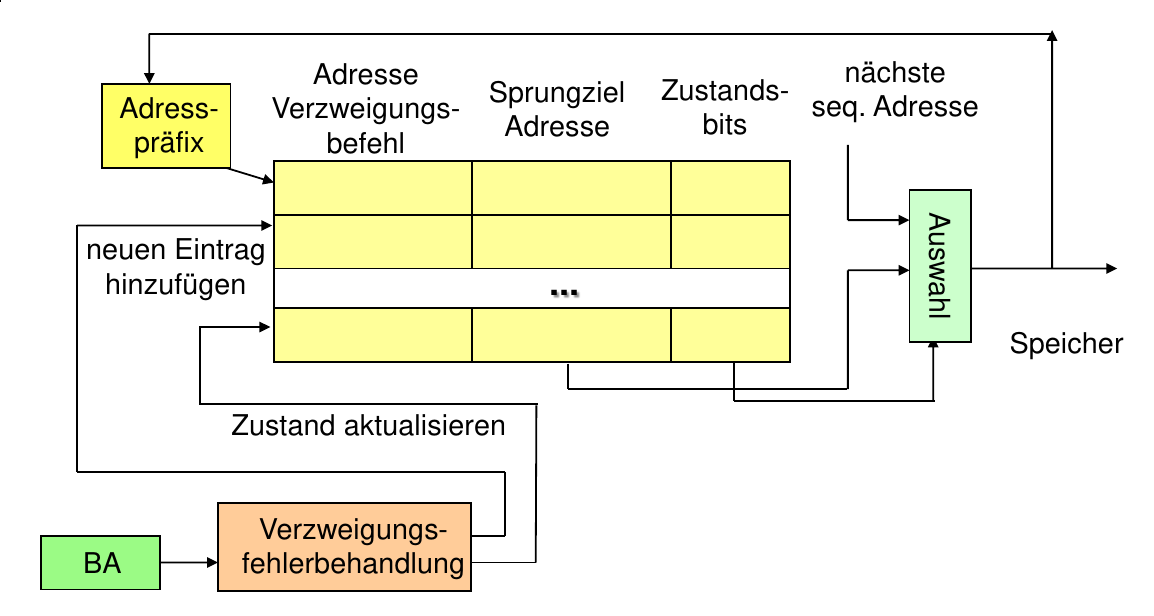
\includegraphics[width=0.9\textwidth]{img/branchtargetbuffer.png}
							\caption{Funktionsweise und Aufbau des branch target buffers}
							\label{fig:hazards}
						\end{figure}
				\end{itemize}
			\item
				Statisch:
				\begin{itemize}
					\item
						Delayed branch: Auswertung des Sprungbefehles vorziehen, evt. dann Sprung ohne Pipeline zu stören ausführen

						Evt. hier TODO
					\item
						Andere statische Gegenmaßnahmen, falls zu vergleichende Register bekannt: zusätzliche Berechnungs-HW, z.B. zusätzliches XOR, berechnung während DE

						Durch zusätzlichen Addierer auch Ziel Wert schon aus Konstante im Befehl und aktuellem BZ berechnen
				\end{itemize}

		\end{itemize}
	\item
		Oder: mehrfache Befehlsausführung: beide Zweige ausführen, nur einen behalten. Was wenn weitere Verzweigungen auftauchen? Struktur-Hazards?
\end{itemize}

\subsubsection{Daten-Hazards}
\begin{itemize}
	\item
		3 Typen von Daten hazards: RAW, WAR, WAW
	\item
		RAW: Instr2 liest einen Operanden den Instr1 noch nicht geschrieben hat.
	\item
		WAR: Instr2 schreibt einen Operanden bevor diesen die früher gestartete Operation Instr1 gelesen hat (überholt Instr1 quasi). Kann in einfachen Pipelines in denen lesen vor schreiben stattfindet nicht passieren
	\item
		WAW: Instr2 schreibt Operanden der von früher gestarteter Operation Instr1 überschrieben wird

\end{itemize}

\subsection{Hazard-Auflösung}
\begin{itemize}
	\item
		Gegenmaßnahme:
		\begin{itemize}
			\item
				Forwarding (berechnete Ergebnisse nicht nur an REgister sondern auch an ALU Eingänge zurück) macht alles viel komplizierter
			\item
				Umordnung Befehlsabfolge in SW (Code Scheduling, wird in EPIC Architekturen gemacht)
			\item
				in HW durch dynamic scheduling (vereinfacht Compilerbau, Code bleibt portierbar, zur Compilezeit unbekannte Abhängigkeiten werden berücksichtigt

				Abweichen vom ursprünglichen Ablaufsplan durch out of order execution oder out of order commits/completion
		\end{itemize}
\end{itemize}
\subsubsection{Scoreboard}
\label{scoreboard}
\begin{itemize}
	\item
		Erlaubt instruktionsausführung ohne Rücksicht auf Reihenfolge im Code
	\item
		Vorraussetzung: keine strukturellen und keine RAW hazards
	\item
		zweiteilige DE/ID Stufe
		\begin{enumerate}
			\item
				Issue stage: befehl bekanntmachen, dekodieren, auf strukturelle Hazards prüfen
			\item
				Read operands: warten bis keine Datenhazards mehr vorhanden, dann lesen der Operanden
		\end{enumerate}
	\item
		Idee stammt vom Großrechner CDC66000 -- mitte der 60er Jahre!
	\item
		Out-of-order-commit kann zu WAR und WAW Hazards führen
		\begin{itemize}
			\item
				Lösung für WAR: entweder Operationen jeweils mit Kopien ihrer Operanden verwalten (tomasulo) oder Register erst schreiben, wenn Operanden gelesen wurden
			\item
				Lösung für WAW: Hazard erkennen und warten bis Konflikt bereinigt ist
		\end{itemize}
	\item
		4 Stufen der Scoreboard verarbeitung:
		\begin{enumerate}
			\item
				Decode 1 und auf strukturelle Hazards checken: checken ob Funktionseinheit frei, keine andere Instruktionen mit selbem Zielregister anhängig (WAW$\lightning$)

				Falls gegeben, OP an Funktionseinheit senden und Scoreboard aktualisieren, falls nicht stalls für aktuelle Instruktionen erzeugen und keine weiteren Instruktionen aktivieren (in order issue)
				
			\item
				Operand lesen: Warten bis keine Datenhazards, dann Lesen der betroffenen Register (decode 2)
				\begin{itemize}
					\item
						Quelloperand ist nutzbar wenn früher aktivierte Instruktion ihn schreibt und die Instruktion endet oder wenn Operandenregister gar nicht erst benutzt wird
					\item
						Ist Quelloperand nutzbar, aktiviert Scoreboard funktionseinheit zum Lesen und Starten der Verarbeitung
					\item
						RAW wird dynamisch aufgelöst, Operationen werden out-of-order executed und gleichzeitig an Funktionseinheiten geschickt
				\end{itemize}
			\item
				OP ausführen. Bei Multizyklus OP wird Scoreboard benachrichtigt, wenn OP beendet
			\item
				Rückschreiben der Ergebnisse. Überprüfen ob WAR vorliegen kann, wenn ja stalls einfügen bis Hazard aufgelöst

		\end{enumerate}
						\begin{figure}[hpbt]
							\centering
							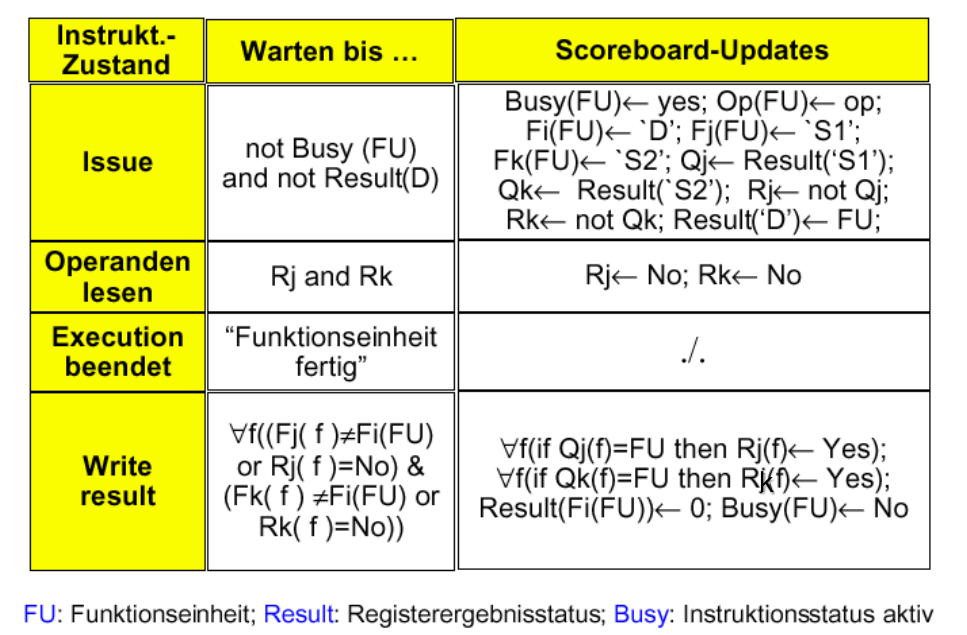
\includegraphics[width=0.7\textwidth]{img/scoreboard.png}
							\caption{Scoreboard Steuerungsalgorithmus, S1 op S2 $\rightarrow$ D, $F_i$ Zielregister, $F_j,F_k$ Quellregister, $Q_j,Q_k$ Funktionseinheiten die Quellregisterdaten erzeugen, $R_j,R_k$, Flags die anzeigen ob $F_j$ oder $F_k$ nutzbar sind}
							\label{fig:hazards}
						\end{figure}
\end{itemize}
\subsubsection{Tomasolu}
\label{tomasolu}

\begin{itemize}
	\item
		KOmbiniert Register-Umbenennung mit Scoreboard um WAW und WAR Hazards zu vermeiden
	\item
		Führt Reservierungseinheiten ein: Steuer und Zwischenspeicher
	\item
		Registerreferenzen in Instruktionen werden durch konkrete Datenwerte oder Zeiger auf ReservierungsStationen ersetzt
	\item
		Resultate von Berechnungen werden nicht über Register sondern über gemeinsamen Datenbus an alle Funktionseinheiten verteilt
	\item
		Load Store sind auch Funktionseinheiten mit Reservierungsstationen
	\item
		Registerergebnisstatus zeigt für jedes Register an, welche FU darauf schreibt
		\begin{figure}[hpbt]
			\centering
			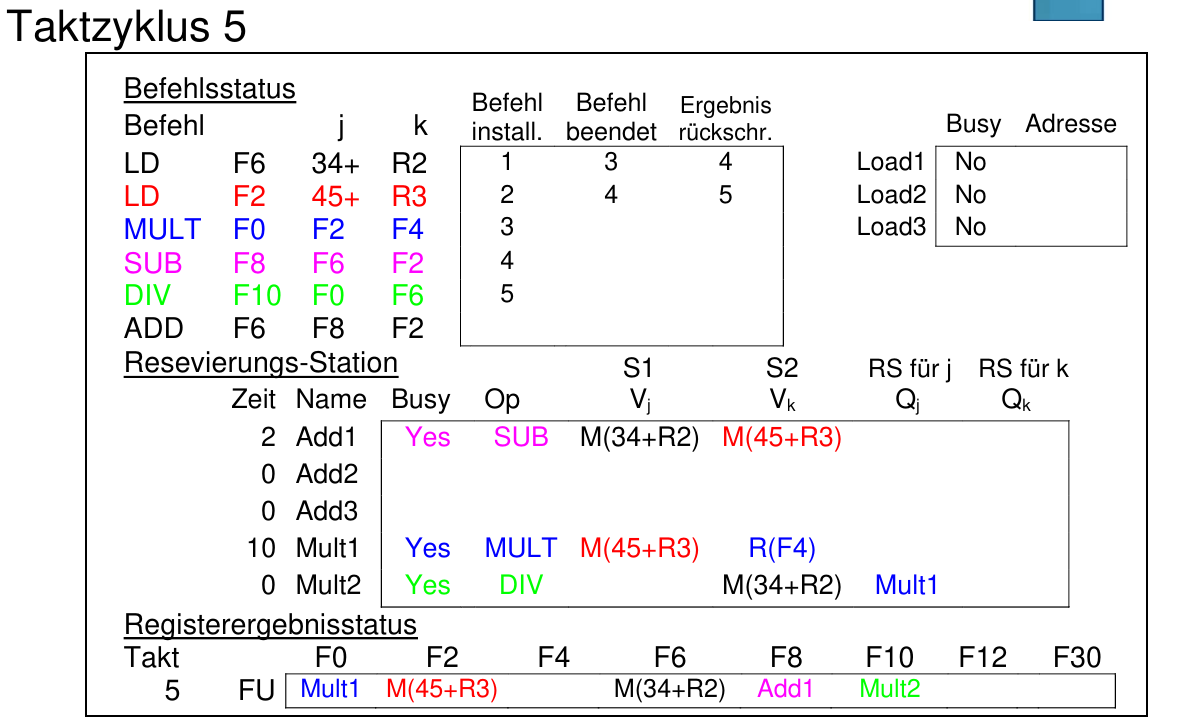
\includegraphics[width=0.9\textwidth]{img/tomasulo.png}
			\caption{}
			\label{fig:tomasulo}
		\end{figure}

	\item
		Vorteil Tomasulo: Vermeidung von wAW und WAR Hazards durch Register Umbenennung/Kopieren, Forwarding
	\item
		Nachteil Tomasulo: mehr HW aufwand, komplexere Kontrolllogik, assoziative Speicherung

\end{itemize}
\subsubsection{Erweiterung um Reorder-Buffer}
\begin{itemize}
	\item
		Ergebnisse kommen in reihenfolge des Codes in den Reorder Buffer
	\item
		Zwischenpuffer um Ergebnisse als in-order-commit zurückzuschreiben
	\item
		Bei Exceptions klar klar, welche Instruktionen abgeschlossen sein dürfen
\end{itemize}
\subsection{Optimale Pipelinetiefe}
\subsection{Cache Architekturen}
\subsubsection{Wiederholung: Cache-Organisation}
\subsubsection{Cache-Ersetzungsstrategien}
\subsubsection{Ausnutzen von Cache-Effekten}
\subsubsection{Cache-Kohärenz}




\newpage
\section{Homogene und heterogene Multikern-Architekturen}
\subsection{Motivation Multikern Architekturen}
\begin{itemize}
	\item
		Warum multicore?
		\begin{itemize}
			\item
				Bis 2002 leistungssteigerung primär durch höhere Taktzahlen
			\item
				Erhöhung der Taktfrequenz stößt an Grenzen (Wärme) \Ra{} Verbesserungen durch intelligentere Architekturen, aber dynamische Sprungvorhersage bereits 95\% Trefferquote, geht jetzt auch nicht mehr viel
		\end{itemize}
	\item
		Mehrere Prozessorkerne auf einem Chip
	\item
		Pollacks Regel:
		\begin{itemize}
			\item
				Rechenleistungszuwachs {\raise.17ex\hbox{$\scriptstyle\sim$}} $\sqrt{\text{Anstieg Komplexität}}$
			\item
				Verdopplung der Logik in Prozessor \ra 40\% mehr Leistung
		\end{itemize}
	\item
		Weitere Vorteile: Einzelkerne an und ausschaltbar, immer optimale Versorgungsspannung und Frequenz, Rechenlast gleichmäßiger Verteilen
	\item
		Umgekehrte  Anwendung der Regel von Pollack: im oberen beherrschabren Energieverbrauchs Spektrum bleiben und Anzahl der Kerne erhöhen (statt $1\times1000000000$ lieber $100\times10000000$ Transistoren)
		\begin{itemize}
			\item
				Leistung nimmt invers quadratisch ab: auf halber Fläche 70\% der Leistung des größeren Systems möglich
			\item
				Leistungsverbrauch pro Kern nimmt linear ab/zu
			\item
				Durchsatz steigt annähernd linear mit größerer Anzahl Kerne
		\end{itemize}
	\item
		Nach Amdahls Law ist Geschwindigkeitszuwachs durch parallelisierung limitiert: Gilt jedoch nur für eine auf allen Kernen laufende Applikation. Häufig jedoch viele Applikationen
	\item
		Roofline Modell:
		\begin{itemize}
			\item
				Wichtige Größe: Operationelle Intensität -- Anzahl der Operationen pro geholtem Byte [Flops/Byte], messgröße für Verkeher zwischen DRAM und Cache
		\end{itemize}
\end{itemize}
\subsection{Leistungsanalyse und -bewertung homogener und heterogener Multikern Prozessoren}
\subsection{Beispiel homogene Multikern-Architekturen}
\subsubsection{Intel Skylake, Haswell, Sandy Bridge}
\subsubsection{ AMD Ryzen}


\subsection{Beispiel heterogene Multikern Architekturen}
\subsubsection{GPGPUs}
\subsubsection{Ausblick: Vielkern-Architekturen}

\subsection{Programmierung homogener und heterogener Multikern-Architekturen}

\newpage
\section{Eingebettete Prozessorachitekturen}
\subsection{Digitale Signalprozessoren}
\subsection{Energiearme eingebettete Prozessoren}
\subsubsection{MIPS}
\subsubsection{ARM}
\subsubsection{RISC-V}

\newpage
\section{Parallelrechnerarchitekturen}


\end{document}
